\documentclass{article}
\usepackage{graphicx}
\usepackage{amsmath}
\usepackage{pgfplots}
\usepackage{physics}
\usepackage{cancel}
\usepackage{enumitem}
\usepackage{txfonts}
\usepackage{multicol}

\pgfplotsset{compat=1.18}

\usepackage[a4paper, top=1cm, bottom=1cm, left=1cm, right=1cm, includehead, includefoot]{geometry}

\begin{document}

\noindent
Math 110B - Calculus \hfill Aaron W. Tarajos
\begin{center}
	\textbf{Midterm Notes}
\end{center}

\noindent\rule{\textwidth}{0.4pt}

\begin{multicols}{2}

\subsubsection*{Trig angles}
    \begin{tabular}{|l|c|c|c|}
        \hline
	Function & $\frac{\pi}{4}(45)$ & $\frac{\pi}{3}(60)$ & $\frac{\pi}{6}(30)$\\
        \hline
	$\sin \theta$ & $\frac{2}{\sqrt2}$ & $\frac{\sqrt 3}{2}$ & $\frac{1}{2}$\\
	$\cos \theta$ & $\frac{2}{\sqrt2}$ & $\frac{1}{2}$ & $\frac{\sqrt{3}}{2}$ \\
	$\tan \theta$ & 1 & $\sqrt{3}$ & $\frac{\sqrt{3}}{3}$ \\
	\hline
    \end{tabular}

\subsubsection*{Work}
\[
	W = \int f(x)\ dx \quad OR \quad W = \int \rho \cdot d \cdot A \ dy
\]

\subsubsection*{Integration by parts}
\[
	\int f(x)g^\prime(x)\ dx = \int f(x)g(x) - \int g(x)f^\prime(x)\ dx
\]

\subsubsection*{Partial Fraction Decomposition}
Given some rational function
\[
	\frac{x+1}{(x+1)(x+3)} = \frac{A}{x+1} + \frac{B}{x+3} \implies x+1 = A(x+3) + B(x+1)
\]
Solve for A and B using a system of equations then integrate. Note if we have a repeat term like $(x+1)^2$ then;
\[
	\frac{x+1}{(x+1)^2(x+3)} = \frac{A}{x+1} + \frac{B}{(x+1)^2} + \frac{C}{x+3}
\]
Then solve as normal

\subsubsection*{Volumes by slices}
\[
	V = \int_{x_1}^{x_2} \pi r^2(x)\ dx \quad \text{OR} \quad V = \int_{x_1}^{x^2} \pi \left(r_1^2 - r_2^2 \right)\ dx
\]

\subsubsection*{Volumes by shells}
\[
	V = \int_{x_1}^{x_2} 2\pi x f(x)\ dx
\]
Note: be careful about the integration bounds and radius, for example,  a slice with $r_1$ of $y=3$ and $r_2$ of $\sec(x) + 1$ rotated about $y=1$ would be\\ $A = \pi \left( (3-1)^2 - (\sec(x) + 1 - 1)^2 \right)$.

\subsubsection*{Trig sub}
\begin{minipage}{0.2\textwidth}
    \begin{tabular}{|l|l|}
        \hline
        Expression & Substitution\\
        \hline
        $\sqrt{a^2-x^2}$ & $x=a\sin\theta$\\
        $\sqrt{a^2+x^2}$ & $x=a\tan\theta$\\
        $\sqrt{x^2-a^2}$ & $x=a\sec\theta$\\
        \hline
    \end{tabular}
\end{minipage}
\begin{minipage}{0.3\textwidth}
    \begin{enumerate}
	\item Draw a triangle
	\item Define the edge lengths using pythagorean theorem
	\item Define trig functions for the triangle
	\item Sovle for $x$ in terms of a trig function and $dx$. Ex;
		\[
			x = \sin \theta (x)
		\]
		\[
			dx = cos \theta\ d \theta
		\]
    \end{enumerate}
\end{minipage}

\subsubsection*{Arc length}
\[
	L = \int_a^b \sqrt{1 + \left(\frac{dy}{dx}\right)^2}\ dx
\]
Derived from pathagorean theorem for the infinite sum of secant lines i.e. $\sqrt{\Delta x^2 + \Delta y^2} = \sqrt{\Delta x^2 + (f^\prime(x)\Delta x)^2}$ factor out $\Delta x$ to obtain the equation.

\subsubsection*{Some other useful antiderivates}
\begin{align*}
	\int \frac{1}{\sqrt{1-x^2}} &= \arcsin x + C \\
	\int -\frac{1}{\sqrt{1-x^2}} &= \arccos x + C \\
	\int \frac{dx}{x^2-a^2} &= \frac{1}{2a} \ln \left| \frac{x-a}{x+a} \right| \\
	\int \frac{dx}{\sqrt{x^2 \pm a^2}} &= \ln \left| x + \sqrt{x^2 \pm a^2} \right| \\
	\int f^{-1}(x) \ dx &= x f^{-1}(x) - (F \circ f^{-1})(x) + C
\end{align*}

\subsubsection*{Surface area}
\[
	S = 2\pi \int_a^b y \sqrt{1+\left( \frac{dy}{dx} \right)^2}\ dx
\]

\subsubsection*{Hydrostatic force}
Pressure is given by
\[
	P = \int_\text{deepest point}^\text{shallow point} \rho \cdot area \cdot depth
\]

where area is width as a function of y and height is $dy$ and $\rho$ is the density.

\subsubsection*{Trig integral tip}
If encountering a form like
\[
	\int \sin^5 x \cos^4 x\ dx
\]
let $u$ be the lower order term and keep one of the higher order terms from the other then convert the rest to match using $1 = \cos^2 x + \sin^2 x$

\end{multicols}

\pagebreak
\begin{multicols}{2}
\section*{Problems that were implied to be on the exam}
\subsection*{Work}
A tank is full of water. Find the work required to pump the water out of the spout. In Exercises 25 and 26 use the fact that water weighs 62.5 lb/ft$^3$.

Draw a circle and use the slice method. The function of the circle is $x^2 + y^2 = 9$ and the volume of each slice is $V = \pi x^2 \Delta y = \pi (9-y^2) \Delta y$. Then the distance is $(4-y)$
\[
	W = \pi \int_{-3}^3 (9-y^2)(4-y)\ dy
\]
Note that its in meters so we can just use 1000 kg/m$^3$ for density of water don't forget to convert mass to weight if using this approach, lb are a unit of weight.

\subsection*{Integration by parts}
\[
	\int e^{2x} \cos(3x)\ dx
\]

\begin{align*}
	\int e^{2x} \cos(3x)\ dx &= \frac{e^{2x} \cos(3x)}{2} - \int -\frac{e^{2x} 3 \sin(3x)}{2}\ dx \\
				 &= \frac{e^{2x} \cos(3x)}{2} + \frac{3}{2}\int e^{2x} \sin(3x)\ dx \\
				 &= \frac{e^{2x} \cos(3x)}{2} + \frac{3}{2}\left[\frac{e^{2x} \sin(3x)}{2} - \frac{3}{2}\int e^{2x} \cos(3x)\ dx \right] \\
				 &= \frac{e^{2x} \cos(3x)}{2} + \frac{3e^{2x} \sin(3x)}{4} - \frac{9}{4}\int e^{2x} \cos(3x)\ dx \\
\end{align*}
Then
\begin{align*}
	\frac{13}{4} \int e^{2x} \cos(3x)\ dx &= \frac{e^{2x} \cos(3x)}{2} + \frac{3e^{2x} \sin(3x)}{4} \\
					      &= \boxed{\frac{2e^{2x} \cos(3x)}{13} + \frac{3e^{2x} \sin(3x)}{13}}
\end{align*}

\subsection*{Trig sub}

\[
	\int \frac{x^2}{\sqrt{9-25x^2}}\ dx
\]

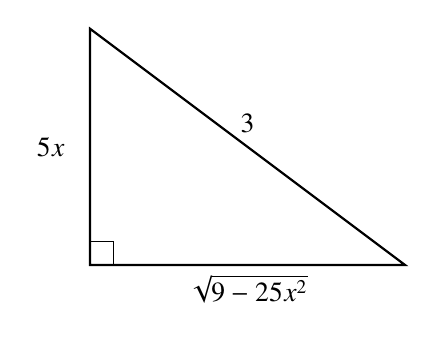
\begin{tikzpicture}
    \draw[thick] (0, 0) -- (4, 0) -- (0, 3) -- cycle;

    \node at (2, -0.3) {$\sqrt{9 - 25x^2}$};
    \node at (-0.5, 1.5) {$5x$};
    \node at (2, 1.8) {$3$};

    \draw (0, 0) rectangle (0.3, 0.3);
\end{tikzpicture}

Let $x = \frac{3}{5} \sin \theta$, $dx = \frac{3}{5} \cos \theta \ d\theta$, and $\sec \theta = \frac{3}{\sqrt{9-25x^2}}$, then;

\begin{align*}
	\int \frac{x^2}{\sqrt{9-25x^2}}\ dx &= \int \left( \frac{3 \sin \theta}{5}\right)^2 \cdot \frac{\sec \theta}{3} \cdot \frac{3}{5}\cos \theta \ d \theta \\
					    &= \int \frac{9}{125} \sin^2 \theta \ d \theta \\
					    &= \frac{9}{125} \int \frac{1-\cos(2 \theta)}{2} \ d \theta \\
					    &= \frac{9}{250} \int 1 - \cos(2 \theta) \ d \theta \\
					    &= \frac{9}{250} \left[ \theta - \frac{\sin 2\theta}{2} \right] + C \\
					    &= \frac{9}{250} \left[ \theta - 2 \sin \theta \cos \theta \right] + C \\
					    &= \frac{9}{250} \left[ arcsin\left(\frac{5x}{3}\right) - 2\left(\frac{5x}{3}\right)\left(\frac{\sqrt{9-25x^2}}{3} \right) \right] + C
\end{align*}

\subsubsection*{Notable tricks if you're stuck}
\begin{enumerate}
	\item You can integrate by parts with $g(x) = 1$
	\item \[ \frac{x^2}{x^2+1} = \frac{x^2 + 1 - 1}{x^2 +1} = 1 - \frac{1}{x^2+1} \]
	\item related to (2) find creative ways to multiply by 1 to create substitutable problems. i.e. $\int \sec \theta$ see below
	\item when doing $u$ sub you can write $x$ as a function of $u$ and sub out remaining $x$ that are unresolved by $\frac{du}{dx}$
\end{enumerate}

\begin{align*}
	\int \sec \theta \ d \theta &= \int \sec \theta \cdot \frac{\sec \theta + \tan \theta}{\sec \theta + \tan \theta} \ d \theta \\
				    &= \int \frac{sec^2 \theta + \sec \theta \tan \theta}{\sec \theta + \tan \theta} \ d \theta \\
				    &= \int \frac{1}{u} \ du \\
				    &= \ln|u| \\
				    &= \ln|\sec \theta + \tan \theta | + C
\end{align*}


\end{multicols}

\end{document}
